\begin{figure}[htbp]
	\centering
	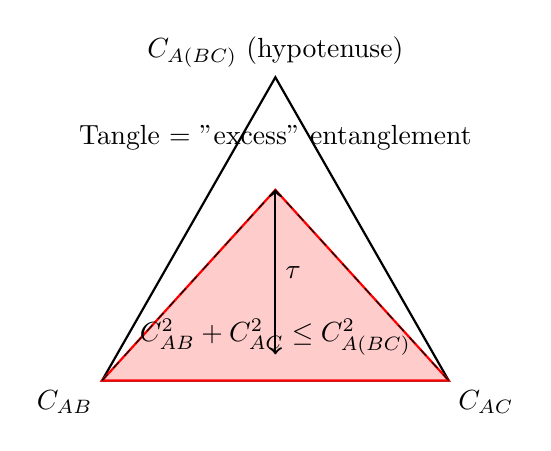
\begin{tikzpicture}[scale=1.1]
		\draw[thick] (0,0) -- (4,0) -- (2,3.5) -- cycle;

		\draw[thick, red, fill=red!20] (0,0) -- (4,0) -- (2,2.2) -- cycle;

		\node at (2,0.5) {$C_{AB}^2 + C_{AC}^2 \leq C_{A(BC)}^2$};

		\node[below left] at (0,0) {$C_{AB}$};
		\node[below right] at (4,0) {$C_{AC}$};
		\node[above] at (2,3.5) {$C_{A(BC)}$ (hypotenuse)};

		\draw[<->, thick] (2,0.3) -- (2,2.2) node[midway, right] {$\tau$};

		\node at (2,2.8) {Tangle = "excess" entanglement};

		\draw[dashed] (4,0) -- (2,2.2);
		\draw[dashed] (0,0) -- (2,2.2);

	\end{tikzpicture}
	\caption{Coffman-Kundu-Wootters (CKW) inequality visualization for three qubits. The triangle inequality shows that the squared entanglement $C_{A(BC)}^2$ (hypotenuse) must be at least as large as the sum of squared pairwise entanglements $C_{AB}^2 + C_{AC}^2$. The tangle $\tau$ represents the genuine tripartite entanglement not captured by pairwise measures. CKW inequality visualization: For three qubits, the squared concurrences satisfy $C_{AB}^2 + C_{AC}^2 \leq C_{A(BC)}^2$. The tangle $\tau = C_{A(BC)}^2 - C_{AB}^2 - C_{AC}^2$ represents the "excess" genuine tripartite entanglement beyond pairwise correlations.}
	\label{fig:ckw-inequality}
\end{figure}
